\documentclass[../main.tex]{subfiles}
\usepackage{graphicx} % Required for including images

\setstretch{0.1} % Adjust spacing for readability

\begin{document}
{\let\clearpage\relax\chapter{Results}}
\vspace{-5pt}

\section{Simulation of an Optical Flat}
\vspace{-15pt}
The evaluation of both ray-tracing and wavefront simulation models in the simulation of optical flats has demonstrated that the integration of these methods provides a clear depiction of optical behaviors. Ray-tracing accurately models the interactions of light waves with optical flats, reflecting the inherent properties of materials and nuances of surface quality. Altough the ray-tracing engine worked, this result was not achieved in this bachelorthesis. Complementary to this, wavefront simulations effectively visualized the propagation and interference of light waves as they interact with surfaces.
\vspace{-15pt}
\subsection{Simulation Results}
\begin{minipage}{\textwidth}
\begin{wrapfigure}{l}{0.3\textwidth}
    \centering
    \vspace{-0.8cm}
    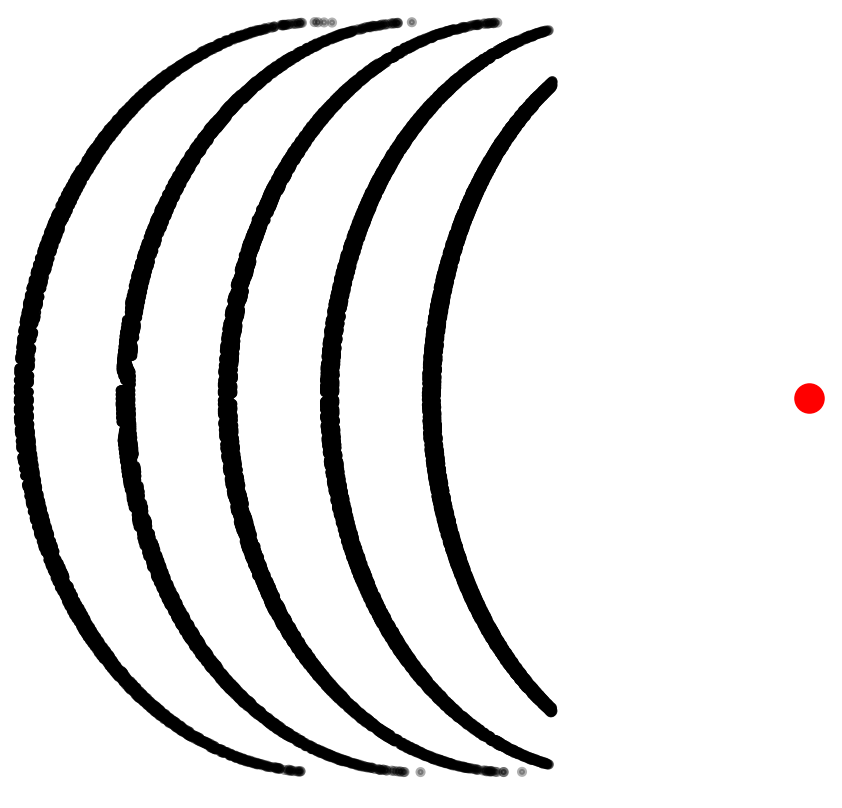
\includegraphics[width=0.3\textwidth]{Images/Results/optical_flat_visualization4}
    \caption{Simulated interference pattern generated by the application. The red dot depicts the place of the hinge of the optical flat. More fringes and more continuity in the fringes can be achieved by adjusting the \texttt{num\_disks} and the \texttt{resolution} parameters.}
    \label{fig:interference}
\end{wrapfigure}
The simulation functionalities within the application were tested to analyze their performance in replicating realistic scenarios. Through the use of the Python-based simulation modules, we were able to perform intersection and visualize interference patterns. Figure \ref{fig:interference} shows a typical simulation output, illustrating the precision and clarity achieved.
\section{Extraction of 3D Surface Shape from Measurements}
Employing the Fourier Transform (FT) method to extract 3D shapes from optical measurements was the key factor to achieve this result. This technique captures fringe patterns embedded with high-frequency carrier fringes and applies Fourier transform techniques to isolate these fringes and recover detailed phase information. The efficacy of this approach is showcased by its ability to convert interference patterns into quantifiable 3D surface maps.

The integration of phase unwrapping and height map calculation features within the GUI simplifies data processing and reduces the time required for analysis. This functionality facilitates the direct transformation of phase data into 3D topographical maps.
\end{minipage}
\subsection{Surface Topography Visualization}
\vspace{-15pt}
The GUI's 3D view tab provides an interactive visualization of reconstructed surfaces. We could manipulate the view to better understand the topographical details of the surface being studied. An example of a reconstructed surface is shown in figure \ref{fig:Cylinder_reconstruction}. At the left, we see the surface of a cylinder with a radius of 2 (figure \ref{fig:Cylinder_sideview}). At the right, you can see the reconstructed surface: planes are used to reconstruct the surface. Although the minimal and maximal values of the reconstruction (respectively -7.72 and 7.82) do not correspond well with the dimensions of the cylinder, we can clearly see that the overall curvature is what we expect to see.\\
\vspace{-15pt}
\begin{figure}[H]
    \centering
    \hfill
    \begin{minipage}{0.49\textwidth}
        \centering
        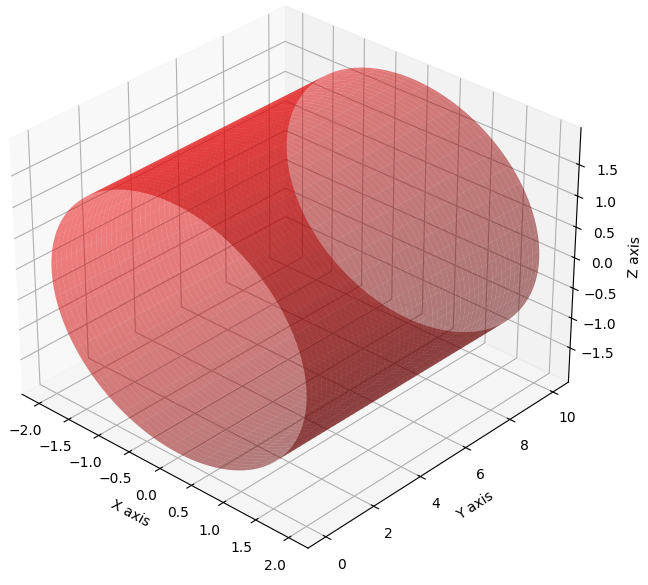
\includegraphics[width=0.95\linewidth]{Images/Results/Cylinder_sideview}
        \caption{Side view of the original cylindrical object, used for simulation input.}
        \label{fig:Cylinder_sideview}
    \end{minipage}
    \hfill
    \begin{minipage}{0.49\textwidth}
        \centering
        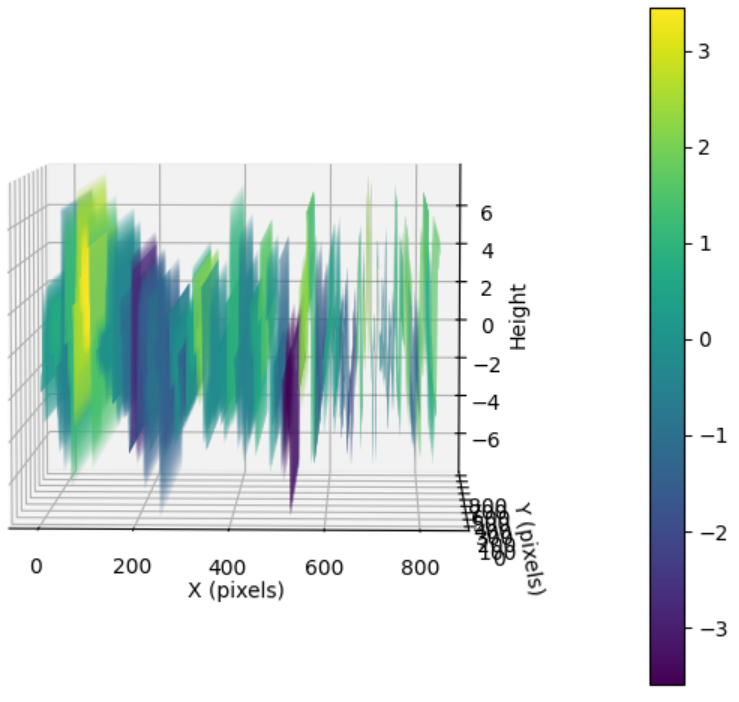
\includegraphics[width=1\linewidth]{Images/Results/Cylinder_reconstruction}
        \caption{3D reconstruction of the cylindrical surface, showing the curvature of surface shape.}
        \label{fig:Cylinder_reconstruction}
    \end{minipage}
\end{figure}
\vspace{-15pt}

Further, we assess a flat surface reconstruction where the fringe patterns indicate a perfect flatness due to straight and parallel lines (see figure \ref{fig:Flat_surface_fringes}). The corresponding reconstruction, depicted figure \ref{fig:Flatsurface_recon}, accurately reflects this flatness. In this case there is no error, because of the fact that the sharpness of the edges of the fringes can't influence the curvature: there is no curvature in a flat surface.
\begin{figure}[H]
    \centering
    \hfill
    \begin{minipage}{0.49\textwidth}
        \centering
        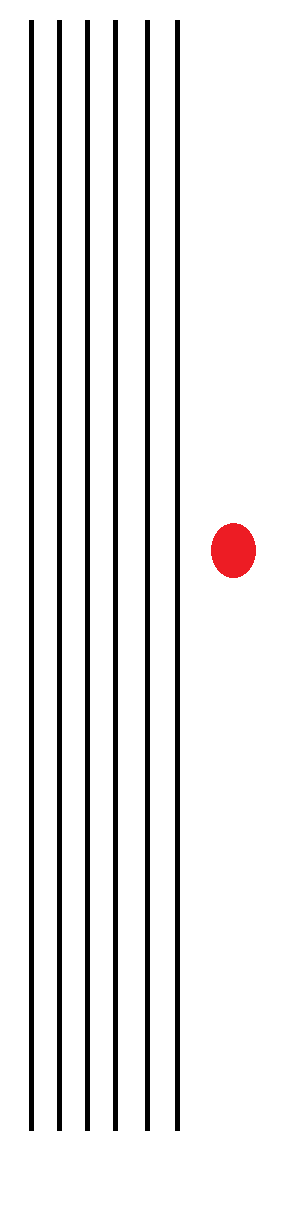
\includegraphics[width=0.2\linewidth]{Images/Results/Flat_surface_fringes}
        \caption{Fringe pattern of a perfectly flat surface. The red dot depicts the place of the hinge of the optical flat.}
        \label{fig:Flat_surface_fringes}
    \end{minipage}
    \hfill
    \begin{minipage}{0.49\textwidth}
        \centering
        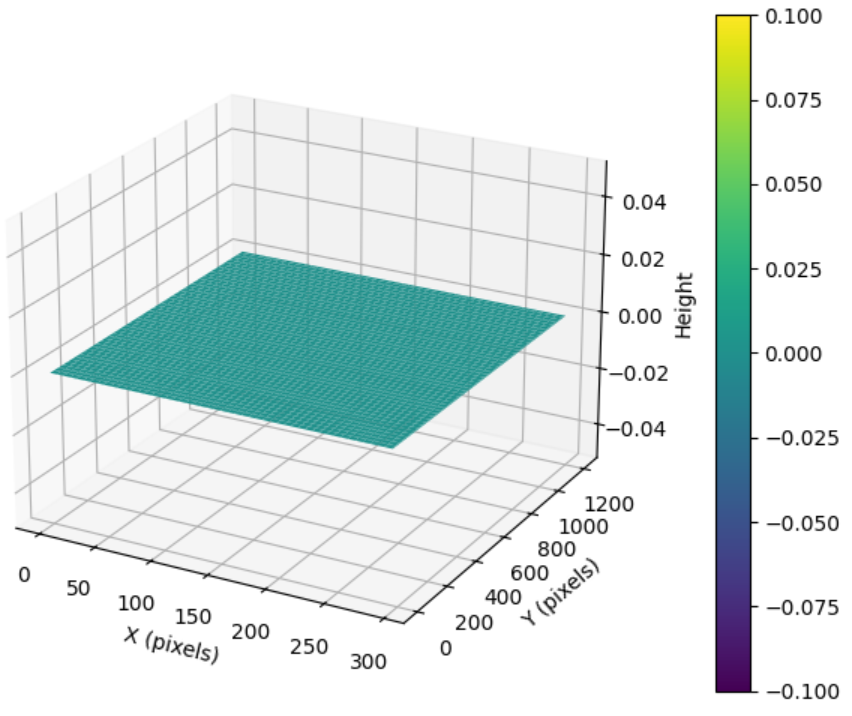
\includegraphics[width=1\linewidth]{Images/Results/Flatsurface_recon}
        \caption{3D reconstruction of the flat surface, showing perfect flatness.}
        \label{fig:Flatsurface_recon}
    \end{minipage}
\end{figure}
\vspace{-15pt}

\section{Representativeness of Simulation and Reconstruction}
\vspace{-15pt}
The quantitative representativeness of the simulations and reconstructions was not evaluated due to lack of time. Instead, we only examined the reconstruction qualitatively by visually comparing the curvature of different shapes. %This could be done by comparing the generated models and extracted data against known standards and real samples. This evaluation indicates that the methods are designed to minimize errors and enhance the accuracy of the simulations. Iterative testing and refining of the simulation parameters should show that they closely align with actual measurements.


\end{document}
